\chapter{Dataset and work done}\label{final}
\section{Dataset}\label{sec2.1}
 The datasets for training and testing the models are taken from the PROMISE repository which consists of 41 different versions of projects. The datasets are taken from 11 open source projects. Data is collected from three or more versions from each of the open source projects.
 
 We used former version of a project as the training data of our models and tested the models' predictions on the latter version for the deep learning regression models developed.
 For anomaly detection, we have taken csv files of all versions and concatenated them to a single dataset, removed the labels and split the training and testing data to 4:1 ratio for the isolation forest model.
 
 The target variable of datasets taken for anomaly prediction had binary values i.e 0 or 1 where 1 meant that a specific data point was flawed and 0 meant that it was unflawed. Whereas, for the deep learning regression problem we took that the datasets which had the target value as the number of faults corresponding to each data point.

\section{Description of Dataset}\label{sec2.2}
The following matrics are proposed by Chidamber and Kemerer, Henderson-Sellers, Martins, QMOOD and Tang et al.
The features in the datasets taken are: 

%Please add the following packages if necessary:
%\usepackage{booktabs, multirow} % for borders and merged ranges
%\usepackage{soul}% for underlines
%\usepackage[table]{xcolor} % for cell colors
%\usepackage{changepage,threeparttable} % for wide tables
%If the table is too wide, replace \begin{table}[!htp]...\end{table} with
%\begin{adjustwidth}{-2.5 cm}{-2.5 cm}\centering\begin{threeparttable}[!htb]...\end{threeparttable}\end{adjustwidth}
\begin{table}[!htp]\centering
\caption{Dataset Features}\label{tab: }
\scriptsize
\begin{tabular}{lrr}\toprule
Abbreviation &Dataset Features \\
CBO &Coupling between objects \\\midrule
RFC &Response for a class \\
LCOM &Lack of cohesion in methods \\
NOC &Number of children \\
DIT &Depth of inheritance \\
WMC &Weighted methods per class \\
Ca &Afferent couplings \\
Ce &Efferent Couplings \\
NPM &Number of public methods \\
DAM &Data Access Metric \\
MOA &Measure of Aggregation \\
MFA &Measure of Functional Abstraction \\
CAM &Cohesion Among Methods of Class \\
AMC &Average Method Complexity \\
LOC &Line of Code \\
CBM &Coupling Between Methods \\
IC &Inheritance Coupling \\
\bottomrule
\end{tabular}
\end{table}

%Please add the following packages if necessary:
%\usepackage{booktabs, multirow} % for borders and merged ranges
%\usepackage{soul}% for underlines
%\usepackage[table]{xcolor} % for cell colors
%\usepackage{changepage,threeparttable} % for wide tables
%If the table is too wide, replace \begin{table}[!htp]...\end{table} with
%\begin{adjustwidth}{-2.5 cm}{-2.5 cm}\centering\begin{threeparttable}[!htb]...\end{threeparttable}\end{adjustwidth}
\begin{table}[!htp]\centering
\caption{Explanation of the features}\label{tab: }
\scriptsize
\begin{tabular}{lrr}\toprule
Abbreviation &Explanation \\
CBO &counts the number of other classes to which a class is coupled with. \\\midrule
RFC &counts the number of external and internal classes. \\
LCOM &measures dissimilarity of methods in a class. \\
NOC &counts the number of descendants of a class. \\
DIT &measures number of ancestor classes. \\
WMC &counts the number of methods in a class weighted by complexity. \\
Ca &counts how many other classes use a given class. \\
Ce &counts the number of classes. a class is dependent upon. \\
NPM &counts the number of public methods in a class. \\
DAM &the number of private methods divided by the total number of methods. \\
MOA &counts the number of abstract data types in a class. \\
MFA &the number of inherited methods divided by total number of methods accessible by its member functions. \\
CAM &based upon the parameters in a method. \\
AMC &counts average size of method in a class. \\
LOC &counts the number of lines of source code. \\
CBM &counts the newly added func- tions with which inherited based methods are coupled. \\
IC &it is based upon inheritance-based coupling. \\
\bottomrule
\end{tabular}
\end{table}

\section{Work done}\label{sec2.3}

This section gives the overview of the work done and includes all the concepts and work done in the experiments. Indetailed explanation about each concept and term used the following subsections will be given the following next two chapters. 

\subsection{Anomaly Detection}
Data files of all the versions of a project are concatenated into a single dataframe and features without unique values are trimmed. The data did not include any null values to handle and the percentage of faulty datapoints was found to be 4.7090517241379315 \%. Applying normalization will result in the outliers not being too distinctive from the rest of the data points, so feature scaling was not applied on the dataset. Scatter plots and distribution plots were obtained of the dataset for each feature and analysed. From the plots, the distinctive behaviour of the defective data points was clearly perceivable. The data set was visualized in 3D and 2D space using t-SNE. We noticed that the data points were not distinctive in 2D or 3D space. So, we went with the earlier finalized features and didn't opt for further feature selection. We removed the labels from our data to treat the problem as unsupervised and split the training and testing data to 4:1 ratio. We used IsolationForest() function from sklearn package for building the model. To evaluate the performance of the model built, we calculated the metrics in confusion matrix and calculated the model accuracy which came out to be 87.70576131687243 \%. 

The detailed flow chart 
of the entire experiment is
given:

 \begin{figure}
\makebox[\textwidth][c]{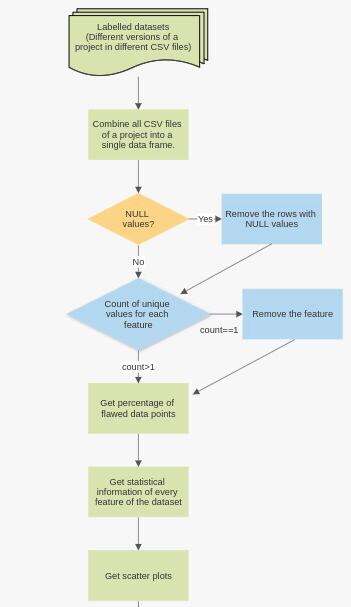
\includegraphics[width=0.6\textwidth]{others/flow1.jpeg}}%
  \caption{Flowchart of the anomaly detection experiment}
  \label{fig:key}
\end{figure}

 \begin{figure}
\makebox[\textwidth][c]{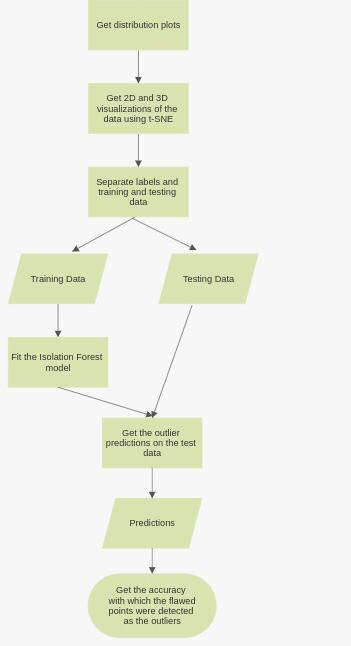
\includegraphics[width=0.6\textwidth]{others/flow2.jpeg}}%
  \caption{Flowchart continuation}
  \label{fig:key}
\end{figure}

\subsection{Regression using Deep Learning}

Exploratory data analysis has been done on the two versions of the project which were taken for training and testing the model. The analysis included checking the presence of null data points, making sure all the features had unique values for the datasets, checking the datatypes of the features and visualizing the scatter plot and frequency distribution of the data for each feature. As per the analysis done, no data cleaning or feature filteration was needed. A specific version ant-1.3 was taken to train the data and ant-1.4 version was taken for testing the models built. Min Max scaling was applied and models' performance were checked with and without different two feature reduction techiniques: SVD and PCA with each taking two different number of components hyperparameter values. Since the data points in the training and testing datasets were very few and might be inadequate for the deep learning models to learn efficiently, we used RandomOverSampler() and SMOTE() functions from imblearn package to increase the size of the data and balance it. The models were developed using tensorflow keras in python. We obtained the training and testing time of the models using the time() function from time package. The predictions obtained were round off to the nearest integer using np.rint() from numpy package because the target value to be predicted was a strict integer. Following the decision in the paper Ridge and Lasso Regression Models for Cross-Version Defect Prediction by Xiaoxing Yang and Wushao Wen we have considered FPA(Fault-percentile-average) and CLC(Cumulative lift chart (also the area under CLC)) as our main model evaluation metrics. At the end of each experiment we have automated the saving of the model weights and results in csv. 

The detailed flow chart of the experiments done for regression using deep learning is given:

 \begin{figure}
\makebox[\textwidth][c]{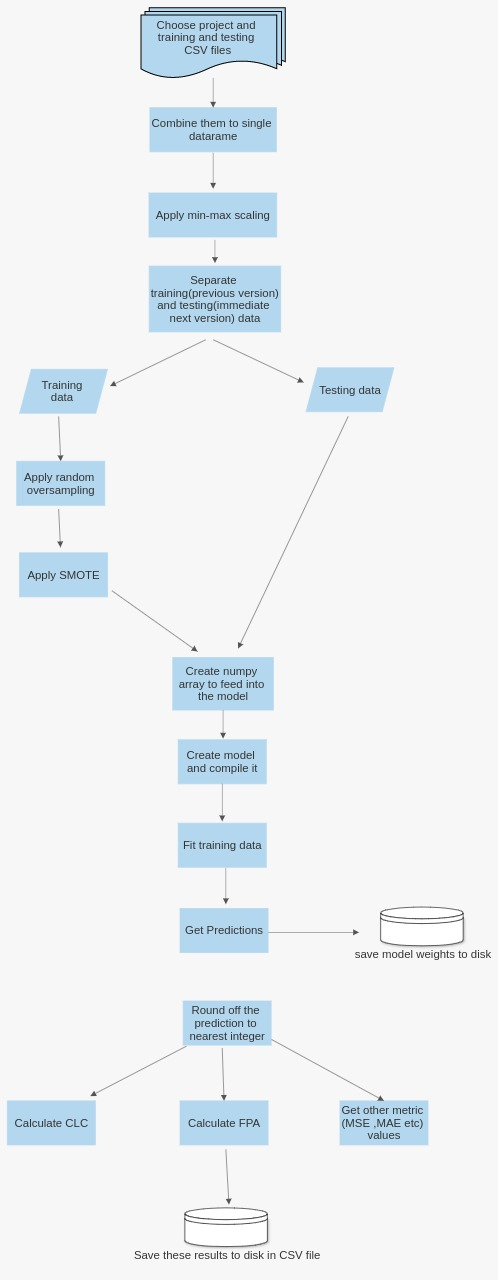
\includegraphics[width=0.6\textwidth]{others/flow_reg.jpeg}}%
  \caption{Flowchart of the anomaly detection experiment}
  \label{fig:key}
\end{figure}